
\section{Introduction}

\vspace{8 pt}

\vspace{8 pt}

\subsection{Background}

\vspace{8 pt}



One challenge that owners of public spaces face is balancing people’s comfort and expended resources. One of the most prominent aspects of comfort relates to temperature and cooling. In open air and semi-open spaces, public space operators need a way to keep people appropriately cooled whilst managing electricity, water, and money. The added exchange of air with the outdoors adds complexity: wind-driven ventilation carries air through openings, so the occupied zone exchanges heat and moisture with its surroundings~\cite{energyplus_wind_ventilation}.

\vspace{4 pt}

Some examples of these spaces include open-sided bus shelters, rail station platforms, stadium concourses, outdoor restaurant patios, concert venues, and covered outdoor airport curbside areas. In the open-sided cases considered here, cooled supply air mixes with outdoor air. We estimate how much of the device-level cooling reaches the occupied zone.

\vspace{4 pt}

These public spaces act like the open air coolers that some convenience stores use. An open refrigerated display case exchanges air with the warmer store environment. Its performance depends on product temperatures, infiltration, case and air-curtain design, and the temperature, humidity, and motion of the surrounding air~\cite{ashrae_refrigeration_2022}. Therefore, a public cooling system should be evaluated by the relief it delivers per unit of energy. 


\vspace{8 pt}

\subsection{Problem Interpretation}
We interpret the cooling comparison and communication tasks in the supplied problem as follows~\cite{comap_2026_problem_b}.

\vspace{8 pt}

\begin{enumerate}

    \item Determine which physical quantities are needed to measure cooling effectiveness in an open-air or semi-open public space.

    \item Develop a physical model that predicts waiting-area temperature, humidity, airspeed, electricity
     consumption, and water consumption for the Fan System, Evaporative Cooler, and Larger Evaporative Cooler.

    \item Estimate the cooling experienced in the waiting area after outlet air mixes with outdoor air.

  \item Convert the modeled environmental conditions into a human-comfort measure that treats temperature,
     humidity, air movement, radiation, clothing, and activity together.

  \item Compare the three cooling systems using both total comfort improvement and comfort improvement per unit
     of electricity.

  \item Determine how evaporative cooling performance changes between dry, humid, and extremely hot weather.
  \item Extend the bus-shelter model to semi-open rail-station waiting areas with different outdoor-air exchange
     rates.

   \item Balance cooling effectiveness against electricity, water consumption, purchase cost, and operational
     uncertainty.

  \item Develop a decision rule that remains useful when the exact future weather condition is unknown.
  \item Test whether the recommendation changes when uncertain inputs are varied.
  \item Produce practical operating guidelines for HiMCM, including when a lower-energy Fan System may be
     preferable to a larger cooling system.

  \item Compare thermal comfort and identify when a separate heat-safety assessment is needed.

\end{enumerate}

\vspace{8 pt}

\subsection{Deliverables}

\vspace{8 pt}
  We present the following deliverables:

\begin{enumerate}

  \item A multizone heat-and-moisture balance model for open-air and semi-open waiting areas.
  \item A psychrometric model for calculating humidity ratio, wet-bulb temperature, evaporative-cooler outlet
     conditions, and water consumption.

  \item A mass-balance check that prevents unbalanced or physically inconsistent airflow networks from being
     accepted.

  \item A thermal-comfort model based on the Gagge two-node representation of the human body~\cite{comf_0112_set,cbe_two_node}.
  \item Standard Effective Temperature estimates for each venue, weather scenario, and cooling system.
  \item Measures of cooling benefit, residual discomfort, and comfort improvement per unit of
     electricity.

  \item Electricity, water, and equipment purchase-cost comparisons.
  \item A minimax-regret decision model that identifies a robust cooling choice across multiple weather
     scenarios.

  \item A sensitivity analysis showing which inputs have the greatest influence on SET, resource use, and the
     recommended system.

  \item A comparison of the Fan System, Evaporative Cooler, and Larger Evaporative Cooler at six bus and rail
     reference venues, with six additional courtyard and airport-canopy cases.

  \item Actionable recommendations for operating cooling systems while balancing comfort, electricity, water,
     and cost.

  \item A memorandum to HiMCM’s Chief Operations Officer and a public-facing blog post explaining how much
     useful cooling is obtained for the energy consumed.


\end{enumerate}

\vspace{8 pt}

\subsection{Justification of Quantities for Measuring Cooling Efficiency}
At its core, cooling efficiency should measure how effectively a system delivers its intended service relative to the resources it consumes. An open freezer case illustrates why electricity consumption alone is insufficient. Its purpose is to maintain food at appropriate temperatures despite continuous heat gains from its surroundings. According to the ASHRAE Handbook—Refrigeration, these gains arise from conduction through the case, thermal radiation, and infiltration of warm, humid air through the opening. Lighting, fans, and defrost systems introduce additional loads. The magnitude of these losses also depends on the case's geometry, air-curtain performance, surrounding temperature and humidity, and external air movement~\cite{ashrae_refrigeration_2022}. In fact, the U.S. Department of Energy found that infiltration alone accounts for approximately 70–80\% of the cooling load in medium-temperature, remote-condensing open refrigerated display cases~\cite{doe_display_cases_2013}. This helps explain why ASHRAE Standard 72 evaluates product temperature performance and refrigeration load alongside energy consumption~\cite{ashrae72_2022_scope}. A fair comparison holds product temperature and storage capacity constant.

For public cooling, the intended service is heat relief for occupants. According to ASHRAE Standard 55, thermal comfort depends on six interacting factors: air temperature, radiant temperature, humidity, airspeed, clothing insulation, and metabolic activity~\cite{ashrae55_2023_scope}. Consequently, measuring only the reduction in air temperature can misrepresent the benefits of different technologies. Fans can improve convective and evaporative heat loss by moving air across the body~\cite{cbe_fans_2023}. Direct evaporative coolers lower dry-bulb temperature while adding moisture; their available temperature reduction decreases as the entering air approaches saturation~\cite{pnnl_evaporative}. Moreover, as with an open freezer, some cooling inevitably dissipates into the surrounding environment. The size of the effectively cooled area, duration of cooling, and number of people benefiting must therefore be considered alongside the magnitude of the thermal improvement.

These observations motivate our model's distinction between cooling effectiveness, the improvement in conditions experienced by occupants, and cooling efficiency, that improvement relative to resource consumption. We quantify the former through changes in Standard Effective Temperature (SET), which combines environmental and personal influences in a human heat-balance calculation~\cite{ashrae_thermal_comfort_2025}. Our implemented comparison uses one reference person and a standardized exposure duration; population weighting would require concurrent occupancy data. We then evaluate this benefit against electricity consumption, while separately reporting water use and purchase cost. The cost comparison uses equipment purchase prices. These quantities are especially important for evaporative systems because evaporation consumes water~\cite{pnnl_evaporative}. Finally, conservation of energy, moisture balances, and physical operating limits constrain the predicted cooling to achievable conditions, and operators need a separate assessment for safe exposure limits.


\subsection{Plan of Action}
We first assemble city weather records, reference equipment specifications, and explicitly labeled venue airflow assumptions. Model I uses a multizone heat-and-moisture balance framework to predict device outlet states and their mixing with outdoor air. Model II converts the resulting environment into SET for a reference occupant. Model III compares comfort loss, resource use, and purchase cost, then applies minimax regret across the three selected weather scenarios. Finally, sensitivity tests examine how uncertain inputs affect the recommendation, and the findings inform the memorandum and blog post.

\begin{figure}[htbp]
    \centering
    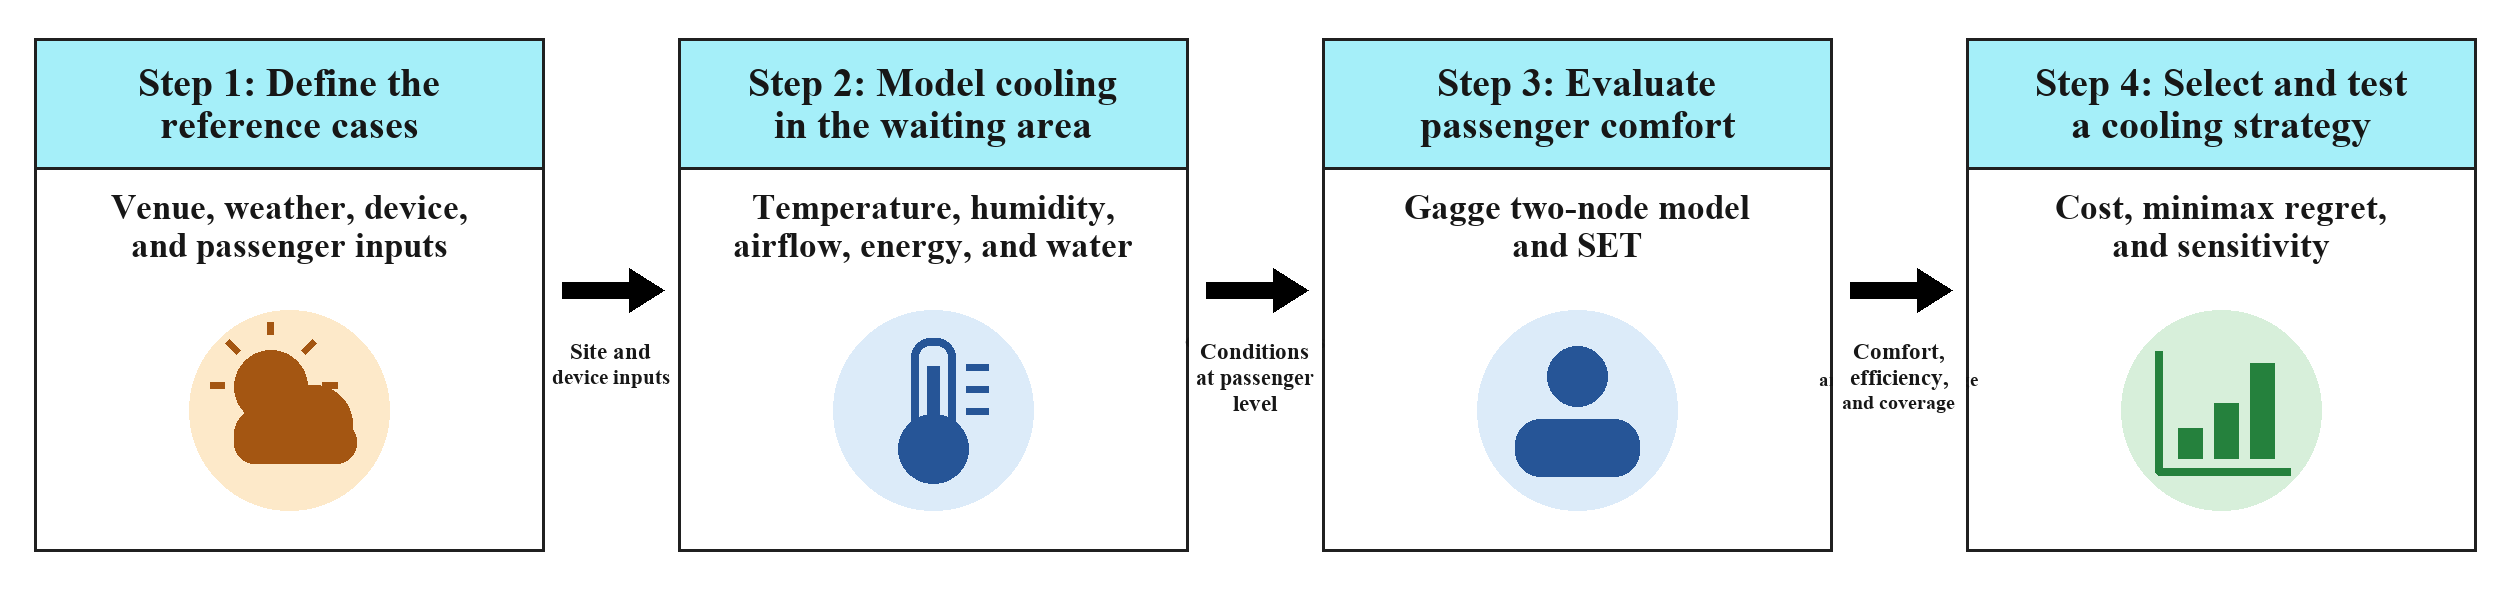
\includegraphics[width=\linewidth]{Images/action_plan_flowchart.png}
    \caption{Flowchart of the action plan.}
    \label{fig:action-plan}
\end{figure}

We used OpenAI Codex to assist with source documentation, calculation checks, and manuscript revisions~\cite{openai_codex_review}.
